% Options for packages loaded elsewhere
\PassOptionsToPackage{unicode}{hyperref}
\PassOptionsToPackage{hyphens}{url}
%
\documentclass[
]{book}
\usepackage{lmodern}
\usepackage{amsmath}
\usepackage{ifxetex,ifluatex}
\ifnum 0\ifxetex 1\fi\ifluatex 1\fi=0 % if pdftex
  \usepackage[T1]{fontenc}
  \usepackage[utf8]{inputenc}
  \usepackage{textcomp} % provide euro and other symbols
  \usepackage{amssymb}
\else % if luatex or xetex
  \usepackage{unicode-math}
  \defaultfontfeatures{Scale=MatchLowercase}
  \defaultfontfeatures[\rmfamily]{Ligatures=TeX,Scale=1}
\fi
% Use upquote if available, for straight quotes in verbatim environments
\IfFileExists{upquote.sty}{\usepackage{upquote}}{}
\IfFileExists{microtype.sty}{% use microtype if available
  \usepackage[]{microtype}
  \UseMicrotypeSet[protrusion]{basicmath} % disable protrusion for tt fonts
}{}
\makeatletter
\@ifundefined{KOMAClassName}{% if non-KOMA class
  \IfFileExists{parskip.sty}{%
    \usepackage{parskip}
  }{% else
    \setlength{\parindent}{0pt}
    \setlength{\parskip}{6pt plus 2pt minus 1pt}}
}{% if KOMA class
  \KOMAoptions{parskip=half}}
\makeatother
\usepackage{xcolor}
\IfFileExists{xurl.sty}{\usepackage{xurl}}{} % add URL line breaks if available
\IfFileExists{bookmark.sty}{\usepackage{bookmark}}{\usepackage{hyperref}}
\hypersetup{
  pdftitle={Untitled},
  pdfauthor={이기준},
  hidelinks,
  pdfcreator={LaTeX via pandoc}}
\urlstyle{same} % disable monospaced font for URLs
\usepackage{color}
\usepackage{fancyvrb}
\newcommand{\VerbBar}{|}
\newcommand{\VERB}{\Verb[commandchars=\\\{\}]}
\DefineVerbatimEnvironment{Highlighting}{Verbatim}{commandchars=\\\{\}}
% Add ',fontsize=\small' for more characters per line
\usepackage{framed}
\definecolor{shadecolor}{RGB}{248,248,248}
\newenvironment{Shaded}{\begin{snugshade}}{\end{snugshade}}
\newcommand{\AlertTok}[1]{\textcolor[rgb]{0.94,0.16,0.16}{#1}}
\newcommand{\AnnotationTok}[1]{\textcolor[rgb]{0.56,0.35,0.01}{\textbf{\textit{#1}}}}
\newcommand{\AttributeTok}[1]{\textcolor[rgb]{0.77,0.63,0.00}{#1}}
\newcommand{\BaseNTok}[1]{\textcolor[rgb]{0.00,0.00,0.81}{#1}}
\newcommand{\BuiltInTok}[1]{#1}
\newcommand{\CharTok}[1]{\textcolor[rgb]{0.31,0.60,0.02}{#1}}
\newcommand{\CommentTok}[1]{\textcolor[rgb]{0.56,0.35,0.01}{\textit{#1}}}
\newcommand{\CommentVarTok}[1]{\textcolor[rgb]{0.56,0.35,0.01}{\textbf{\textit{#1}}}}
\newcommand{\ConstantTok}[1]{\textcolor[rgb]{0.00,0.00,0.00}{#1}}
\newcommand{\ControlFlowTok}[1]{\textcolor[rgb]{0.13,0.29,0.53}{\textbf{#1}}}
\newcommand{\DataTypeTok}[1]{\textcolor[rgb]{0.13,0.29,0.53}{#1}}
\newcommand{\DecValTok}[1]{\textcolor[rgb]{0.00,0.00,0.81}{#1}}
\newcommand{\DocumentationTok}[1]{\textcolor[rgb]{0.56,0.35,0.01}{\textbf{\textit{#1}}}}
\newcommand{\ErrorTok}[1]{\textcolor[rgb]{0.64,0.00,0.00}{\textbf{#1}}}
\newcommand{\ExtensionTok}[1]{#1}
\newcommand{\FloatTok}[1]{\textcolor[rgb]{0.00,0.00,0.81}{#1}}
\newcommand{\FunctionTok}[1]{\textcolor[rgb]{0.00,0.00,0.00}{#1}}
\newcommand{\ImportTok}[1]{#1}
\newcommand{\InformationTok}[1]{\textcolor[rgb]{0.56,0.35,0.01}{\textbf{\textit{#1}}}}
\newcommand{\KeywordTok}[1]{\textcolor[rgb]{0.13,0.29,0.53}{\textbf{#1}}}
\newcommand{\NormalTok}[1]{#1}
\newcommand{\OperatorTok}[1]{\textcolor[rgb]{0.81,0.36,0.00}{\textbf{#1}}}
\newcommand{\OtherTok}[1]{\textcolor[rgb]{0.56,0.35,0.01}{#1}}
\newcommand{\PreprocessorTok}[1]{\textcolor[rgb]{0.56,0.35,0.01}{\textit{#1}}}
\newcommand{\RegionMarkerTok}[1]{#1}
\newcommand{\SpecialCharTok}[1]{\textcolor[rgb]{0.00,0.00,0.00}{#1}}
\newcommand{\SpecialStringTok}[1]{\textcolor[rgb]{0.31,0.60,0.02}{#1}}
\newcommand{\StringTok}[1]{\textcolor[rgb]{0.31,0.60,0.02}{#1}}
\newcommand{\VariableTok}[1]{\textcolor[rgb]{0.00,0.00,0.00}{#1}}
\newcommand{\VerbatimStringTok}[1]{\textcolor[rgb]{0.31,0.60,0.02}{#1}}
\newcommand{\WarningTok}[1]{\textcolor[rgb]{0.56,0.35,0.01}{\textbf{\textit{#1}}}}
\usepackage{longtable,booktabs}
\usepackage{calc} % for calculating minipage widths
% Correct order of tables after \paragraph or \subparagraph
\usepackage{etoolbox}
\makeatletter
\patchcmd\longtable{\par}{\if@noskipsec\mbox{}\fi\par}{}{}
\makeatother
% Allow footnotes in longtable head/foot
\IfFileExists{footnotehyper.sty}{\usepackage{footnotehyper}}{\usepackage{footnote}}
\makesavenoteenv{longtable}
\usepackage{graphicx}
\makeatletter
\def\maxwidth{\ifdim\Gin@nat@width>\linewidth\linewidth\else\Gin@nat@width\fi}
\def\maxheight{\ifdim\Gin@nat@height>\textheight\textheight\else\Gin@nat@height\fi}
\makeatother
% Scale images if necessary, so that they will not overflow the page
% margins by default, and it is still possible to overwrite the defaults
% using explicit options in \includegraphics[width, height, ...]{}
\setkeys{Gin}{width=\maxwidth,height=\maxheight,keepaspectratio}
% Set default figure placement to htbp
\makeatletter
\def\fps@figure{htbp}
\makeatother
\setlength{\emergencystretch}{3em} % prevent overfull lines
\providecommand{\tightlist}{%
  \setlength{\itemsep}{0pt}\setlength{\parskip}{0pt}}
\setcounter{secnumdepth}{5}
\usepackage{booktabs}
\ifluatex
  \usepackage{selnolig}  % disable illegal ligatures
\fi
\usepackage[]{natbib}
\bibliographystyle{apalike}

\title{Untitled}
\author{이기준\footnote{국가교육통계연구본부장, \href{mailto:standard@kedi.re.kr}{\nolinkurl{standard@kedi.re.kr}}}}
\date{2021-02-16}

\begin{document}
\maketitle

{
\setcounter{tocdepth}{1}
\tableofcontents
}
\hypertarget{uxc2dcuxacc4uxc5f4-uxb370uxc774uxd130}{%
\chapter{시계열 데이터}\label{uxc2dcuxacc4uxc5f4-uxb370uxc774uxd130}}

우리는 연도별 학생수, 날짜별 기온 변화 등과 같이 시간의 흐름에 따라 수집된 데이터를 흔히 볼 수 있다. 특히 가장 흔하게 볼 수 있는 시계열 데이터는 주식시장에서 볼 수 있는데 주식에 관련된 대부분의 데이터가 시계열 데이터이다. 시계열 데이터는 과거의 데이터 패턴을 분석하여 유사한 데이터 흐름이 지속된다는 가정하에 미래 특정한 기간동안의 데이터 흐름을 분석하기 위해 사용되고 있다.

시계열 데이터는 일련의 시간간의 흐름에 따라 기록되는 데이터들의 집합이기 때문에 인접한 시간의 데이터간의 상관관계가 존재한다. 최근 우리나라는 저출산 고령화 사회에 접어들었다고 한다. 우리나라의 출생아수는 지속적으로 줄고 있다고 하는데 갑자기 늘거나 갑자기 줄거나 하지는 않는다. 이와 같이 과거의 데이터가 현재의 데이터에 영향을 주는 경향을 자기상관이라고 하는데 비시계열 데이터에 비교해서 이 자기 상관성이 시계열 데이터의 큰 특징이라고 할 수 있다.

최근 머신러닝이 발달함에 따라 데이터를 기반으로 예측하는 알고리즘들이 많이 소개되고 사용되고 있다. 그 알고리즘들은 regression, classification, clustering 등의 알고리즘을 사용하여 모델을 생성하고 새로운 데이터가 주어졌을때 해당 모델을 통해 예측 값을 산출해내는 작업을 수행한다. 그러나 시계열 데이터는 앞서 설명한 자기 상관과 같은 특수성으로 인해 일반적으로 머신러닝에서 사용하는 알고리즘들을 사용하지 않고 시계열 데이터를 분석하기 위한 Arima, Exponential Smoothing 등의 방법을 사용하여 데이터를 모델링 한 후 특별한 입력값이 없어도 미래 시간의 흐름에 따라 일련의 예측값을 생성할 수 있다는 점에서 머신러닝 알고리즘과 차이가 있다.

그러나 최근에는 머신러닝 알고리즘을 시계열 데이터에 적용하여 미래 예측을 하는 방법도 속속 소개되고 있고 Facebook에서는 자사에서 개발한 시계열 데이터 분석 알고리즘(Prophet)을 소개하는 등 시계열 데이터에 대한 예측 알고리즘도 발전하고 있다.

\hypertarget{uxc815uxc758}{%
\section{정의}\label{uxc815uxc758}}

시계열(Time Series) 데이터는 일정한 시간에 따른 순차적 정보량을 기록한 데이터이다 .

기록되는 순차적 정보량은 여러 측정치가 가능한데 대부분의 경우 가격, 온도, 인구수 등 수치적 측정치나 특성(Feature) 등이 기록되지만 이들을 핸들링하는 인덱스는 시간형 타입으로 설정되거나 시간을 나타낼 수 있는 타입으로 설정되어야 한다.

시계열 데이터는 과거 데이터의 흐름에 따른 경향성(Trend), 계절별이나 특정 기간의 경과에 따른 데이터의 반복적 흐름(Seasonality), 주기적인 데이터의 증감(Cyclic)를 발견하여 향후 불확실한 미래의 데이터 흐름을 예측(Forecasting)하는데 활용할 수 있다.

\hypertarget{uxd2b9uxc131}{%
\section{특성}\label{uxd2b9uxc131}}

\hypertarget{uxace0uxc815uxb41c-uxc2dcuxac04-uxb3c5uxb9bduxbcc0uxc218}{%
\subsection{고정된 시간 독립변수}\label{uxace0uxc815uxb41c-uxc2dcuxac04-uxb3c5uxb9bduxbcc0uxc218}}

일반적으로 데이터 분석시에는 독립변수와 종속변수간의 관계를 분석하는 것이 목적인 경우가 많다.

종속변수의 행동을 예측하기 위해서는 하나 혹은 여러개의 독립변수가 필요하고 이들간의 관계성을 도출함으로서 향후 독립변수에 따라 종속변수의 예측값을 도출하게 되는데 아래의 예제와 같이 자동차의 속도와 제동거리간에는 그래프 상으로 양의 상관관계를 보이고 있음. 이 예제에서는 제동거리를 종속변수로, 자동차 속도를 독립변수로 분석하였다.

그러나 \textbf{시계열 데이터의 독립변수 중 하나는 시간으로 고정됨}. 따라서 시계열 데이터는 타 변수와의 상관관계 없이도 자신 스스로 종속변수이자 독립변수로 분석될 수 있다.

시계열 데이터를 구축하는데 중요한 요소는 시간 간격이 동일해야 한다는 점임. 예를 들어 매시간, 매일, 매월, 매분기, 매년 등 간격이 일정해야 시계열 데이터를 다루기 위한 다양한 함수들에 적용이 가능함. 다만 간격이 일정하더라도 결측치에 의해 모든 간격의 데이터가 기록되지 않은 데이터에 대해 시계열 데이터를 만들고 그래프를 그릴 수는 있으나 예측에 적용하기 위해서는 일정한 간격의 데이터를 갖추는 것이 더 효과적이다.

\hypertarget{uxc790uxae30-uxc0c1uxad00uxad00uxacc4}{%
\subsection{자기 상관관계}\label{uxc790uxae30-uxc0c1uxad00uxad00uxacc4}}

시계열 데이터는 과거의 자기 자신의 데이터와의 상관관계가 존재하는 성질이다.

일반적으로 상관관계는 서로 다른 두개의 변수간의 영향성을 살펴보지만 자기 상관관계는 자기 자신의 n차 지연(lag) 데이터(현재보다 n번째 과거 데이터)와 현재 데이터간의 상관관계가 발생함을 의미한다.

\hypertarget{uxcd94uxc138-uxacbduxd5a5uxc131trend}{%
\subsection{추세 경향성(Trend)}\label{uxcd94uxc138-uxacbduxd5a5uxc131trend}}

시계열 데이터는 장기적으로 점차 증가하거나 점차 감소하는 추세에 대한 경향성을 보이는 경우가 있다.

추세 경향성은 시간의 흐름에 따라 나타나는 인구, 경기, 기술, 환경 등의 변화에 따라 영향을 받는 데이터의 중장기적인 지속적 데이터의 변동을 말하는데 시간축에 따라 발생하는 데이터 변동에 대한 그래프에서 확인이 가능한데 이 변동성을 선형회귀로 단정하여 예측하지 않도록 주의해야 한다.

추세 경향성을 선형회귀로 분석할 때는 앞서 언급한 자기 상관관계가 있는지를 먼저 확인한 후에 적용해야 하며 자기 상관관계가 있는 경우에는 선형회귀보다 다른 시계열 분석방법을 활용하는 방법을 고민해야 한다.

\hypertarget{uxacc4uxc808uxc131seasonality-uxc21cuxd658uxc131cyclic}{%
\subsection{계절성(Seasonality), 순환성(Cyclic)}\label{uxacc4uxc808uxc131seasonality-uxc21cuxd658uxc131cyclic}}

시계열 데이터는 중장기적인 추세경향성외에 데이터가 달력(Calender)상의 날짜나 기간에 따라 주기적으로 변화하거나 장기적인 시간의 흐름에 따라 오르거나 내리는 추세가 반복되는 변동성을 가지는 경우가 있다.

계절성은 봄, 여름, 가을, 겨울과 같은 계절, 일, 주, 월, 분기와 같은 기간의 변화에 따라 주기적으로 변동하는 시계열 성질을 말하고, 순환성은 일정한 기간의 특징없이 데이터의 변동성이 반복되거나 1년을 넘겨 주기적으로 발생하는 데이터의 반복성을 말함

계절성과 순환성은 혼동되는 경우가 많다. 계절성은 주기가 고정된 기간에 대한 순환성이고 순환성은 변동적 기간에 대한 순환성이고 일반적으로 순환성의 주기가 계절성 주기보다 길기 때문에 계절성은 언제쯤 데이터 피크(Peak)가 나타날지 예측이 가능하나 순환성은 데이터 피크에 대한 예측이 어려운 성질이 있다.

\hypertarget{uxbd88uxd655uxc2e4uxc131uncertainty}{%
\subsection{불확실성(Uncertainty)}\label{uxbd88uxd655uxc2e4uxc131uncertainty}}

시계열 모델의 해석에는 반드시 불확실성에 대한 고려가 수반되어야 함. 시계열 분석을 통해 예측된 미래 데이터는 사용된 모델에 적합한 확률 분포 모델(Probability Distribution)을 통한 신뢰구간이 같이 제공되어 평가되어야 한다.

대부분의 시계열 모델은 불확실성을 표현하기 위한 신뢰구간의 산출이 가능한데 시계열 예측은 예측 기간이 길수록 예측의 신뢰구간이 점점 넓어지게 된다.

\hypertarget{uxc2dcuxacc4uxc5f4-uxb370uxc774uxd130-uxd0c0uxc785-uxbc0f-import}{%
\chapter{시계열 데이터 타입 및 Import}\label{uxc2dcuxacc4uxc5f4-uxb370uxc774uxd130-uxd0c0uxc785-uxbc0f-import}}

Placeholder

\hypertarget{uxb0a0uxc9dcuxc2dcuxac04-uxb370uxc774uxd130-uxd074uxb798uxc2a4}{%
\section{날짜/시간 데이터 클래스}\label{uxb0a0uxc9dcuxc2dcuxac04-uxb370uxc774uxd130-uxd074uxb798uxc2a4}}

\hypertarget{date-class}{%
\subsection{Date class}\label{date-class}}

\hypertarget{posixct-posixlt-data-class}{%
\subsection{POSIXct, POSIXlt data class}\label{posixct-posixlt-data-class}}

\hypertarget{yearmon-yearqtr-class}{%
\subsection{yearmon, yearqtr class}\label{yearmon-yearqtr-class}}

\hypertarget{uxb0a0uxc9dc-uxc2dcuxac04-uxd3ecuxb9f7}{%
\subsection{날짜, 시간 포맷}\label{uxb0a0uxc9dc-uxc2dcuxac04-uxd3ecuxb9f7}}

\hypertarget{uxc2dcuxacc4uxc5f4-uxd328uxd0a4uxc9c0-uxbc0f-uxb370uxc774uxd130-uxac1duxccb4object}{%
\section{시계열 패키지 및 데이터 객체(Object)}\label{uxc2dcuxacc4uxc5f4-uxd328uxd0a4uxc9c0-uxbc0f-uxb370uxc774uxd130-uxac1duxccb4object}}

\hypertarget{ts}{%
\subsection{ts}\label{ts}}

\hypertarget{zoo}{%
\subsection{zoo}\label{zoo}}

\hypertarget{xts}{%
\subsection{xts}\label{xts}}

\hypertarget{tsibble}{%
\subsection{tsibble}\label{tsibble}}

\hypertarget{modeltime}{%
\subsection{modeltime}\label{modeltime}}

\hypertarget{uxc2dcuxacc4uxc5f4-uxb370uxc774uxd130-importuxc758-uxbc29uxbc95}{%
\section{시계열 데이터 Import의 방법}\label{uxc2dcuxacc4uxc5f4-uxb370uxc774uxd130-importuxc758-uxbc29uxbc95}}

\hypertarget{uxd30cuxc77cuxc5d0uxc11c-uxc2dcuxacc4uxc5f4-uxb370uxc774uxd130uxb85c-uxc77duxc5b4uxb4e4uxc774uxb294-uxbc29uxbc95}{%
\subsection{파일에서 시계열 데이터로 읽어들이는 방법}\label{uxd30cuxc77cuxc5d0uxc11c-uxc2dcuxacc4uxc5f4-uxb370uxc774uxd130uxb85c-uxc77duxc5b4uxb4e4uxc774uxb294-uxbc29uxbc95}}

\hypertarget{uxc9c1uxc811-uxc2dcuxacc4uxc5f4-uxb370uxc774uxd130-uxd0c0uxc785uxc73cuxb85c-uxc77duxc5b4uxb4e4uxc774uxb294-uxbc29uxbc95}{%
\subsection{직접 시계열 데이터 타입으로 읽어들이는 방법}\label{uxc9c1uxc811-uxc2dcuxacc4uxc5f4-uxb370uxc774uxd130-uxd0c0uxc785uxc73cuxb85c-uxc77duxc5b4uxb4e4uxc774uxb294-uxbc29uxbc95}}

\hypertarget{uxc2e4uxc2b5-uxb370uxc774uxd130-uxc0dduxc131}{%
\section{실습 데이터 생성}\label{uxc2e4uxc2b5-uxb370uxc774uxd130-uxc0dduxc131}}

\hypertarget{uxc6d4uxbcc4-uxb370uxc774uxd130---uxacbduxc81cuxd65cuxb3d9-uxc778uxad6cuxc870uxc0ac-uxc0b0uxc5c5uxbcc4-uxcde8uxc5c5uxc790uxc218}{%
\subsection{월별 데이터 - 경제활동 인구조사 산업별 취업자수}\label{uxc6d4uxbcc4-uxb370uxc774uxd130---uxacbduxc81cuxd65cuxb3d9-uxc778uxad6cuxc870uxc0ac-uxc0b0uxc5c5uxbcc4-uxcde8uxc5c5uxc790uxc218}}

\hypertarget{uxc77cuxbcc4-uxb370uxc774uxd130---uxcf54uxb85cuxb098-uxd655uxc9c4uxc790-uxc218}{%
\subsection{일별 데이터 - 코로나 확진자 수}\label{uxc77cuxbcc4-uxb370uxc774uxd130---uxcf54uxb85cuxb098-uxd655uxc9c4uxc790-uxc218}}

\hypertarget{uxc2dcuxacc4uxc5f4-visualization}{%
\chapter{시계열 Visualization}\label{uxc2dcuxacc4uxc5f4-visualization}}

Placeholder

\hypertarget{data.frame-ggplot2-uxd328uxd0a4uxc9c0}{%
\section{data.frame : ggplot2 패키지}\label{data.frame-ggplot2-uxd328uxd0a4uxc9c0}}

\hypertarget{xts-xts-uxd328uxd0a4uxc9c0}{%
\section{xts : xts 패키지}\label{xts-xts-uxd328uxd0a4uxc9c0}}

\hypertarget{ts-forecast-uxd328uxd0a4uxc9c0}{%
\section{ts : forecast 패키지}\label{ts-forecast-uxd328uxd0a4uxc9c0}}

\hypertarget{tsibble-feasts-uxd328uxd0a4uxc9c0}{%
\section{tsibble : feasts 패키지}\label{tsibble-feasts-uxd328uxd0a4uxc9c0}}

\hypertarget{data.frame-timetk-uxd328uxd0a4uxc9c0}{%
\section{data.frame : timetk 패키지}\label{data.frame-timetk-uxd328uxd0a4uxc9c0}}

\hypertarget{uxc2dcuxacc4uxc5f4-uxb370uxc774uxd130-handling}{%
\chapter{시계열 데이터 Handling}\label{uxc2dcuxacc4uxc5f4-uxb370uxc774uxd130-handling}}

Placeholder

\hypertarget{uxc2dcuxacc4uxc5f4-uxb370uxc774uxd130-uxc815uxbcf4-uxb2e4uxb8e8uxae30}{%
\section{시계열 데이터 정보 다루기}\label{uxc2dcuxacc4uxc5f4-uxb370uxc774uxd130-uxc815uxbcf4-uxb2e4uxb8e8uxae30}}

\hypertarget{uxc2dcuxacc4uxc5f4-uxc815uxbcf4-uxcd94uxcd9c}{%
\subsection{시계열 정보 추출}\label{uxc2dcuxacc4uxc5f4-uxc815uxbcf4-uxcd94uxcd9c}}

\hypertarget{uxc2dcuxacc4uxc5f4-uxb370uxc774uxd130-uxc5f0uxc0b0}{%
\subsection{시계열 데이터 연산}\label{uxc2dcuxacc4uxc5f4-uxb370uxc774uxd130-uxc5f0uxc0b0}}

\hypertarget{uxc2dcuxacc4uxc5f4-uxb370uxc774uxd130-uxbc18uxc62cuxb9bc}{%
\subsection{시계열 데이터 반올림}\label{uxc2dcuxacc4uxc5f4-uxb370uxc774uxd130-uxbc18uxc62cuxb9bc}}

\hypertarget{uxc2dcuxacc4uxc5f4-uxb370uxc774uxd130-grouping}{%
\subsection{시계열 데이터 Grouping}\label{uxc2dcuxacc4uxc5f4-uxb370uxc774uxd130-grouping}}

\hypertarget{uxc2dcuxacc4uxc5f4-uxb370uxc774uxd130-ohlc}{%
\subsection{시계열 데이터 OHLC}\label{uxc2dcuxacc4uxc5f4-uxb370uxc774uxd130-ohlc}}

\hypertarget{uxc2dcuxacc4uxc5f4-uxb370uxc774uxd130-rolling}{%
\subsection{시계열 데이터 Rolling}\label{uxc2dcuxacc4uxc5f4-uxb370uxc774uxd130-rolling}}

\hypertarget{uxc2dcuxacc4uxc5f4-uxb370uxc774uxd130-filtering}{%
\subsection{시계열 데이터 Filtering}\label{uxc2dcuxacc4uxc5f4-uxb370uxc774uxd130-filtering}}

\hypertarget{uxc2dcuxacc4uxc5f4-uxb370uxc774uxd130-uxc751uxc6a9-uxc0acuxb840}{%
\section{시계열 데이터 응용 사례}\label{uxc2dcuxacc4uxc5f4-uxb370uxc774uxd130-uxc751uxc6a9-uxc0acuxb840}}

\hypertarget{uxc6d4uxbcc4-uxbd84uxae30uxbcc4-uxc5f0uxbcc4-uxd569uxacc4}{%
\subsection{월별, 분기별, 연별 합계}\label{uxc6d4uxbcc4-uxbd84uxae30uxbcc4-uxc5f0uxbcc4-uxd569uxacc4}}

\hypertarget{uxc6d4uxbcc4-uxbd84uxae30uxbcc4-uxc5f0uxbcc4-uxc99duxac10uxb7c9}{%
\subsection{월별, 분기별, 연별 증감량}\label{uxc6d4uxbcc4-uxbd84uxae30uxbcc4-uxc5f0uxbcc4-uxc99duxac10uxb7c9}}

\hypertarget{uxc6d4-uxbe44uxc911-uxbc31uxbd84uxc728-uxc5f0-uxbe44uxc911-uxbc31uxbd84uxc728}{%
\subsection{월 비중 백분율, 연 비중 백분율}\label{uxc6d4-uxbe44uxc911-uxbc31uxbd84uxc728-uxc5f0-uxbe44uxc911-uxbc31uxbd84uxc728}}

\hypertarget{uxc6d4uxbcc4-uxbd84uxae30uxbcc4-uxc5f0uxbcc4-uxb204uxc801uxd569uxacc4}{%
\subsection{월별, 분기별, 연별 누적합계}\label{uxc6d4uxbcc4-uxbd84uxae30uxbcc4-uxc5f0uxbcc4-uxb204uxc801uxd569uxacc4}}

\hypertarget{uxb3d9uxc6d4uxbcc4-uxb3d9uxbd84uxae30uxbcc4-uxb3d9uxb144uxbcc4-plot}{%
\subsection{동월별, 동분기별, 동년별 Plot}\label{uxb3d9uxc6d4uxbcc4-uxb3d9uxbd84uxae30uxbcc4-uxb3d9uxb144uxbcc4-plot}}

\hypertarget{uxc2dcuxacc4uxc5f4-forecasting-part-i---uxae30uxcd08uxcee8uxc149}{%
\chapter{시계열 forecasting Part I - 기초컨셉}\label{uxc2dcuxacc4uxc5f4-forecasting-part-i---uxae30uxcd08uxcee8uxc149}}

Placeholder

\hypertarget{uxc815uxc0c1uxc131stationary-uxbe44uxc815uxc0c1uxc131non-stationary}{%
\section{정상성(Stationary), 비정상성(Non-Stationary)}\label{uxc815uxc0c1uxc131stationary-uxbe44uxc815uxc0c1uxc131non-stationary}}

\hypertarget{uxc9c0uxc5f0laguxc640-uxcc28uxbd84difference}{%
\section{지연(Lag)와 차분(Difference)}\label{uxc9c0uxc5f0laguxc640-uxcc28uxbd84difference}}

\hypertarget{acfuxc640-pacf}{%
\section{ACF와 PACF}\label{acfuxc640-pacf}}

\hypertarget{uxc801uxd569uxac12fitted-value-uxc640-uxc794uxcc28residuals}{%
\section{적합값(fitted value) 와 잔차(residuals)}\label{uxc801uxd569uxac12fitted-value-uxc640-uxc794uxcc28residuals}}

\hypertarget{uxbc31uxc0c9-uxc7a1uxc74cwhite-noise}{%
\section{백색 잡음(White Noise)}\label{uxbc31uxc0c9-uxc7a1uxc74cwhite-noise}}

\hypertarget{uxc2dcuxacc4uxc5f4-uxbd84uxd574decomposition}{%
\section{시계열 분해(Decomposition)}\label{uxc2dcuxacc4uxc5f4-uxbd84uxd574decomposition}}

\hypertarget{uxc815uxc0c1uxc131-uxd14cuxc2a4uxd2b8}{%
\section{정상성 테스트}\label{uxc815uxc0c1uxc131-uxd14cuxc2a4uxd2b8}}

\hypertarget{uxacc4uxc808uxc131-plotinguxacfc-uxd14cuxc2a4uxd2b8}{%
\section{계절성 ploting과 테스트}\label{uxacc4uxc808uxc131-plotinguxacfc-uxd14cuxc2a4uxd2b8}}

\hypertarget{uxc2dcuxacc4uxc5f4-forecasting-part-ii---uxc2dcuxacc4uxc5f4-uxc608uxce21-uxbaa8uxb378}{%
\chapter{시계열 forecasting Part II - 시계열 예측 모델}\label{uxc2dcuxacc4uxc5f4-forecasting-part-ii---uxc2dcuxacc4uxc5f4-uxc608uxce21-uxbaa8uxb378}}

Placeholder

\hypertarget{simple-uxbaa8uxb378}{%
\section{Simple 모델}\label{simple-uxbaa8uxb378}}

\hypertarget{uxd3c9uxade0-uxbaa8uxb378forecastmeanf}{%
\subsection{평균 모델(forecast::meanf)}\label{uxd3c9uxade0-uxbaa8uxb378forecastmeanf}}

\hypertarget{uxb2e8uxc21cnaive-uxbaa8uxb378}{%
\subsection{단순(Naive) 모델}\label{uxb2e8uxc21cnaive-uxbaa8uxb378}}

\hypertarget{uxacc4uxc808uxc131-uxb2e8uxc21cseasonal-naive-uxbaa8uxb378}{%
\subsection{계절성 단순(Seasonal Naive) 모델}\label{uxacc4uxc808uxc131-uxb2e8uxc21cseasonal-naive-uxbaa8uxb378}}

\hypertarget{random-work-uxbaa8uxb378}{%
\subsection{Random Work 모델}\label{random-work-uxbaa8uxb378}}

\hypertarget{simple-uxbaa8uxb378-uxbe44uxad50}{%
\subsection{Simple 모델 비교}\label{simple-uxbaa8uxb378-uxbe44uxad50}}

\hypertarget{regression-uxbaa8uxb378}{%
\section{Regression 모델}\label{regression-uxbaa8uxb378}}

\hypertarget{tslm-uxd568uxc218forecast-uxd328uxd0a4uxc9c0}{%
\subsection{tslm 함수(forecast 패키지)}\label{tslm-uxd568uxc218forecast-uxd328uxd0a4uxc9c0}}

\hypertarget{plot_time_series_regression-uxd568uxc218timetk-uxd328uxd0a4uxc9c0}{%
\subsection{plot\_time\_series\_regression 함수(timetk 패키지)}\label{plot_time_series_regression-uxd568uxc218timetk-uxd328uxd0a4uxc9c0}}

\hypertarget{uxc9c0uxc218-uxd3c9uxd65cexponential-smoothing-uxbaa8uxb378}{%
\section{지수 평활(Exponential Smoothing) 모델}\label{uxc9c0uxc218-uxd3c9uxd65cexponential-smoothing-uxbaa8uxb378}}

\hypertarget{uxb2e8uxc21c-uxc9c0uxc218-uxd3c9uxd65c-uxbaa8uxb378simple-exponentail-smoothing-model}{%
\subsection{단순 지수 평활 모델(Simple Exponentail Smoothing Model)}\label{uxb2e8uxc21c-uxc9c0uxc218-uxd3c9uxd65c-uxbaa8uxb378simple-exponentail-smoothing-model}}

\hypertarget{forecastses-uxd568uxc218}{%
\subsubsection{forecast::ses() 함수}\label{forecastses-uxd568uxc218}}

\hypertarget{statsholtwinters-uxd568uxc218}{%
\subsubsection{stats::HoltWinters() 함수}\label{statsholtwinters-uxd568uxc218}}

\hypertarget{uxd640uxd2b8holt-uxbaa8uxb378}{%
\subsection{홀트(Holt) 모델}\label{uxd640uxd2b8holt-uxbaa8uxb378}}

\hypertarget{forecastholt-uxd568uxc218}{%
\subsubsection{forecast::holt() 함수}\label{forecastholt-uxd568uxc218}}

\hypertarget{statsholtwinters-uxd568uxc218-1}{%
\subsubsection{stats::HoltWinters() 함수}\label{statsholtwinters-uxd568uxc218-1}}

\hypertarget{uxd640uxd2b8-uxc708uxd130holt-winter-uxbaa8uxb378}{%
\subsection{홀트-윈터(Holt-Winter) 모델}\label{uxd640uxd2b8-uxc708uxd130holt-winter-uxbaa8uxb378}}

\hypertarget{forecasthw-uxd568uxc218}{%
\subsubsection{forecast::hw() 함수}\label{forecasthw-uxd568uxc218}}

\hypertarget{statsholtwinters-uxd568uxc218-2}{%
\subsubsection{stats::HoltWinters() 함수}\label{statsholtwinters-uxd568uxc218-2}}

\hypertarget{ets-uxbaa8uxb378}{%
\subsection{ETS 모델}\label{ets-uxbaa8uxb378}}

\hypertarget{arima-uxbaa8uxb378}{%
\section{ARIMA 모델}\label{arima-uxbaa8uxb378}}

\hypertarget{uxc790uxae30uxd68cuxadc0uxbaa8uxb378autoregressive-model}{%
\subsection{자기회귀모델(AutoRegressive Model)}\label{uxc790uxae30uxd68cuxadc0uxbaa8uxb378autoregressive-model}}

\hypertarget{uxc774uxb3d9uxd3c9uxade0-uxbaa8uxb378moving-average-model}{%
\subsection{이동평균 모델(Moving Average Model)}\label{uxc774uxb3d9uxd3c9uxade0-uxbaa8uxb378moving-average-model}}

\hypertarget{arima-uxbaa8uxb378-uxacb0uxc815}{%
\subsection{ARIMA 모델 결정}\label{arima-uxbaa8uxb378-uxacb0uxc815}}

\hypertarget{seasonal-arima-uxbaa8uxb378}{%
\subsection{Seasonal ARIMA 모델}\label{seasonal-arima-uxbaa8uxb378}}

\hypertarget{tbats-uxbaa8uxb378}{%
\section{TBATs 모델}\label{tbats-uxbaa8uxb378}}

\hypertarget{prophet-uxbaa8uxb378}{%
\section{prophet 모델}\label{prophet-uxbaa8uxb378}}

\hypertarget{neural-network-uxbaa8uxb378}{%
\section{Neural Network 모델}\label{neural-network-uxbaa8uxb378}}

\hypertarget{uxc2dcuxacc4uxc5f4-forecasting-part-iii---uxc2dcuxacc4uxc5f4-uxbd84uxc11d-framework}{%
\chapter{시계열 forecasting Part III - 시계열 분석 Framework}\label{uxc2dcuxacc4uxc5f4-forecasting-part-iii---uxc2dcuxacc4uxc5f4-uxbd84uxc11d-framework}}

Placeholder

\hypertarget{uxc131uxb2a5uxbd84uxc11d-uxc9c0uxc218}{%
\section{성능분석 지수}\label{uxc131uxb2a5uxbd84uxc11d-uxc9c0uxc218}}

\hypertarget{rmseroot-means-squaread-error}{%
\subsection{RMSE(Root Means Squaread Error)}\label{rmseroot-means-squaread-error}}

\hypertarget{mae}{%
\subsection{MAE}\label{mae}}

\hypertarget{mpe}{%
\subsection{MPE}\label{mpe}}

\hypertarget{mape}{%
\subsection{MAPE}\label{mape}}

\hypertarget{fable}{%
\section{fable}\label{fable}}

\hypertarget{modeltime-1}{%
\section{modeltime}\label{modeltime-1}}

\hypertarget{linear_reg-uxd568uxc218tidymodels-parsnip-modeltime-uxd328uxd0a4uxc9c0}{%
\subsection{linear\_reg 함수(tidymodels, parsnip, modeltime 패키지)}\label{linear_reg-uxd568uxc218tidymodels-parsnip-modeltime-uxd328uxd0a4uxc9c0}}

\hypertarget{r-markdown}{%
\section{R Markdown}\label{r-markdown}}

This is an R Markdown document. Markdown is a simple formatting syntax for authoring HTML, PDF, and MS Word documents. For more details on using R Markdown see \url{http://rmarkdown.rstudio.com}.

When you click the \textbf{Knit} button a document will be generated that includes both content as well as the output of any embedded R code chunks within the document. You can embed an R code chunk like this:

\begin{Shaded}
\begin{Highlighting}[]
\FunctionTok{summary}\NormalTok{(cars)}
\end{Highlighting}
\end{Shaded}

\begin{verbatim}
##      speed           dist       
##  Min.   : 4.0   Min.   :  2.00  
##  1st Qu.:12.0   1st Qu.: 26.00  
##  Median :15.0   Median : 36.00  
##  Mean   :15.4   Mean   : 42.98  
##  3rd Qu.:19.0   3rd Qu.: 56.00  
##  Max.   :25.0   Max.   :120.00
\end{verbatim}

\hypertarget{including-plots}{%
\section{Including Plots}\label{including-plots}}

You can also embed plots, for example:

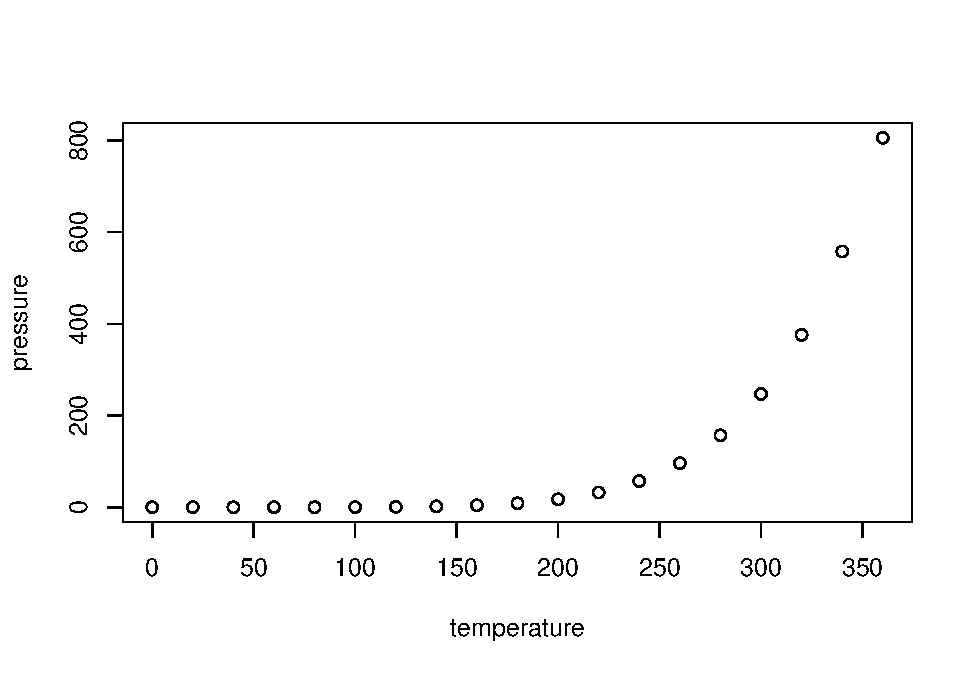
\includegraphics{t_files/figure-latex/pressure-1.pdf}

Note that the \texttt{echo\ =\ FALSE} parameter was added to the code chunk to prevent printing of the R code that generated the plot.

  \bibliography{book.bib,packages.bib}

\end{document}
